\documentclass{../template/llncs}
%
\usepackage{url}
\RequirePackage[hyphenbreaks]{breakurl} % allow hyphenation in URLs
\usepackage{amsmath} % use equations
\RequirePackage[utf8]{inputenc} % support Umlauts and special characters
\usepackage{microtype} % use space more efficiently and hyphenate smarter: all in all looks a lot sexier
\usepackage{listings} % allow source code environments
\usepackage{latexsym} % allows special symbols
\usepackage{graphicx} % enebles figures
\graphicspath{ {content/images/} }
%
\title{Formal Methods for multi-agent systems}
\author{Sergey Dedukh}
\institute{University of Koblenz and Landau}
\tocauthor{ }
%
\begin{document}
\maketitle

\section{Introduction and motivation}
An important part of artificial intelligence research deals with autonomous agents acting in environments which are not or only partially known to the agents in the beginning. Allowing agents to reason about their knowledge and interacting with the environment is tackled by different programming methods. This technical report introduces the two logic programming languages GOLOG and FLUX. The basic structure of each language will be shown together with examples to ease understanding. In the first section the situation calculus will be presented. It is a logic formalism GOLOG builds upon. The two subsequent sections~\ref{golog} and \ref{flux} cover GOLOG and FLUX respectively. This report closes with a conclusion drawn from the features of GOLOG and FLUX regarding a multi-agent scenario with incomplete knowledge.


\section{Theoretical background}
To formalize the concepts of multi agent systems different types of logics are used, such as propositional, modal, temporal and dynamic logics. I this section these logics, their properties and introduced operators will be briefly discussed. Describing the details about interpretations and models of each individual logic is not the purpose of this section and is left out for further reading.

Propositional logic is the simplest one and serves as a fundament for logics discussed further in this section. It is used for representing factual information and in our case is most suitable to model the agent's environment. Formulas in this logic language consist of atomic propositions (known facts about the world) and truth-functional connectives: $\land,\lor,\neg,\rightarrow$ which denote "and" "or" "not" and "implies" respectively. \cite{Enderton_72} 

Modal logic extends propositional logic by introducing two different modes of truth: possibility and necessity. In the study of agents, it is used to give
meaning to concepts such as belief and knowledge. Syntactically modal operators in modal logic languages are defined as $\Diamond$  for possibility and 
$\Box$ for necessity. The semantics of modal logics is traditionally given in terms of sets of the so-called possible worlds. A world here can be interpreted as a possible state of affairs or sequence of states of affairs (history). Different worlds can be related via a binary accessibility relation, which tells us which worlds are are within the realm of possibility from the standpoint of a given world. In the sense of the accessibility relation a condition is assumed possible if it is true somewhere in the realm of possibility and it is assumed necessary if it is true everywhere in the realm of possibility. \cite{Saul_63}

Dynamic logic is also can be referred to as modal logic of action. It adds differen atomic actions to the logic language. In our case atomic actions may be represented as actions that agents can perform directly. This makes dynamic logic very flexible and useful for distributed artificial intelligence systems. Necessity and possibility operators of dynamic logic are based upon the kinds of actions available. \cite{Kozen_90}

Temporal logic is the logic of time. There are several variations of this logic such as:
\begin{itemize}
  \item Linear or Branching: single course of history or multiple courses of history.
  \item Discrete or Dense: discrete steps(like natural numbers) or always having intermediate steps (like real numbers).
  \item Moment-based or Period-based: atoms of time are points or intervals.
\end{itemize}
We will concentrate on discrete moment-based models with linear past, but consider both linear and branching futures.

Linear temporal logic introduces several important operators. $p\cup q$ is true at a moment $t$ on a path, if and only if $q$ holds at a future moment on
the given path and $p$ holds on all moments between $t$ and the selected occurrence of $q$. $Fp$ means that $p$ holds sometimes in the future on the given path. $Gp$ means that $p$ always holds in the future on the given path. $Xp$ means that $p$ holds in the next moment. $Pq$ means that $q$ held in a past moment. \cite{Singh_99}
%
\begin{figure}[h!]
\caption{An example branching structure of time}
\centering
\includegraphics[width=0.6\textwidth]{branching_logic.png}
\label{fig:branching_time}
\end{figure}

Branching temporal and action logic is built on top of both dynamic and linear temporal logics and captures the essential properties of actions and time that are of value in specifying agents. It also adds several specific branching-time operators. $A$ denotes "in all paths at the present moment". The present moment here is the moment at which a given formula is evaluated. $E$ denotes "in some path at the present moment". The reality operator $R$ denotes "in the real path at the present moment". Figure \ref{fig:branching_time} illustrates the example of branching time for two interacting agents.



\section{Formal methods for a single agent}
For modeling intelligent agents quite often used so-called BDI concept. BDI here stands for three cognitive specifications of agents: beliefs, desires, intensions. To model logic of these specifications we will need to introduce several modal operators: $Bel$ for beliefs, $Des$ for desires, $Int$ for intensions and $K_h$ for know how. Considering these operators, for example, the mental state of an agent who desires to win the lottery and intends to buy a lottery ticket sometime, but does not believe that he will ever win can be represented by the following formula: $DesAFwin \land IntEFbuy \land \neg BelAFwin$. For simplification in future we will consider only those desires which are mutually consistent. Such desires are usually called goals.

It is important to note several important properties of intensions, which should be maintained by all agents\cite{Singh_92}:
\begin{enumerate}
  \item Satisfiability: $xIntp\rightarrow EFp$. This means that if $p$ is intended by $x$, then it occurs eventually on some path. Intension following this condition is assumed satisfiable.
  \item Temporal consistency: $(xIntp \land xIntq)\rightarrow xInt(Fp \land Fq)$. This requires that if an agent intends $p$ and intends $q$, then it  (implicitly) intends achieving them in some undetermined temporal order: $p$ before $q$, $q$ before $p$, or both simultaneously.
  \item Persistence does not entail success: $EG((xIntp) \land \neg p)$ is satisfiable. This is quite intuitive: just because an agent persists with an intention does not mean that it will succeed.
  \item Persist while succeeding. This constraint requires that agents desist from revising their intentions as long as they are able to proceed properly.
\end{enumerate}

The introduced above concepts may be used in each of two roles of formal methods introduced earlier. There are two mostly used reasoning techniques to decide agent's actions: theorem proving and model checking. The first one is more complex in terms of calculations, when the second one is more practical, but it requires additional inputs, though it does not prove to be a problem in several cases.

Considering the practical implementation, the architecture of abstract BDI-interpreter can be described as follows. The inputs to the system are called events, and are received via an event queue. Events can be external or internal for the system. Based on its current state and input events the system selects and executes options, corresponding to some plans. The interpreter continually performs the following: determines available options, deliberates to commit some options, updates its state and executes chosen atomic actions, after that it updates the event queue and eliminates the options which already achieved or no longer possible.
%
\begin{lstlisting}
BDI-Interpreter
initialize_state();
do
    options := option-generator(event-queue, B, G, I);
    selected-options := deliberate(options, B, G, I);
    update-intentions(selected-options, I);
    execute(I);
    get-new-external-events();
    drop-successful-attitudes(B, G, I);
    drop-impossible-attitudes(B, G, I);
until quit.
\end{lstlisting}

As was mentioned above options are usually represented by plans. Plans consist of of the name or type, the body usually specified by a plan graph, invocation condition (triggering event), precondition specifying when it may be selected and add list with delete list, specifying which atomic propositions to be believed after successful plan execution. Intentions in this case may be represented as hierarchically related plans.

Getting back to the algorithm and assuming plans as options, the option generator may look like the following.
Given a set of trigger events from the event queue, the option generator iterates through the plan library and returns those plans whose invocation condition
matches the trigger event and whose preconditions are believed by the agent.
%
\begin{lstlisting}[mathescape]
option-generator(trigger-events, B, G ,I)
options := {};
for trigger-event $\in$ trigger-events do
    for plan $\in$ plan-library do
        if matches(invocation(plan, trigger-event) then
            if provable(precondition(plan), B) then
                options := options $\cup$ plan;
return options.
\end{lstlisting}

Deliberation of options should conform with the execution time constraints, therefor under certain circumstances random choice might be appropriate. Sometimes lengthy deliberation becomes possible by introducing metalevel plans into plan library, which form intentions towards some particular plans.
%
\begin{lstlisting}[mathescape]
deliberate(options)
if length(options) $\leq$ 1 then return options;
else metalevel-options :=
            option-generator(b-add(option-set(options)));
    selected-options := deliberate(metalevel-options);
    if null(selected-options) then
        return random-choice(options);
    else return selected-options.
\end{lstlisting}


\section{Formal methods for multiple agents}
Coordination is one of the core functionalities needed by multiagent systems. Especially when different agents autonomous and have different roles and possible actions. 

One of the approaches developed by Singh \cite{Singh_97} represents each agent as a small skeleton, which includes only the events or
transitions made by the agent that are significant for coordination. The core of the architecture is the idea that agents should have limited knowledge about designs of other agents. This limited knowledge is called a significant events of the agent. Events can be of the four main types:
\begin{itemize}
  \item flexible, which can be delayed or omitted,
  \item inevitable, which can be only delayed,
  \item immediate, which agent willing to perform immediately,
  \item triggerable, which the agent performs based on external events.
\end{itemize}
These events are organized into skeletons that characterize the coordination behavior of agents. The coordination service is independent of the exact skeletons or events used by agents in a multiagent system.

To specify coordinations a variant of linear-time temporal language with some restrictions is used. For that purpose two temporal operators are introduced: $\cdot$ - before operator, and $\bigodot$ - the operator of concatenation of two time traces, first of which is finite. Such special logic allows a variety of different relationships to be captured. 

\section{Conclusion}
In this last part, we reflect on the actual competition as well as our own work.
First, \autoref{con:competition} presents the setup and procedure of the competition, as well as the results.
Moreover, some general observations we made while monitoring the behaviour of our agents throughout the matches are given in this section.
\autoref{con:learned} builds upon these observations by explaining in more detail the things we noticed and the conclusions we were able to draw from them.
This section also discusses more general lessons we have learned while developing our multi-agent system.

\subsection{Competition results}
The competition took place on two dates (15th and 17th of September) and each team had to play three times against all other teams. Each simulation consisted of a total of 400 steps and the team with the highest score at the end got three points for a victory. The overall score is the sum over all 400 step scores. The score per step is composed of points for zones plus achievement points. Since the strategy of team "MaKo" was to extensively buy upgrades for the artillery agent", most of the earned achievement points were consumed and therefore did not count towards the step score. Figure \autoref{dis:achievement_points} shows the progress of achievement points over time. As one can see, the achievement points of team "MaKo" go up and down due to the buying actions whereas the the points of the other team increase constantly. 
\begin{figure}[ht]
	\centering
	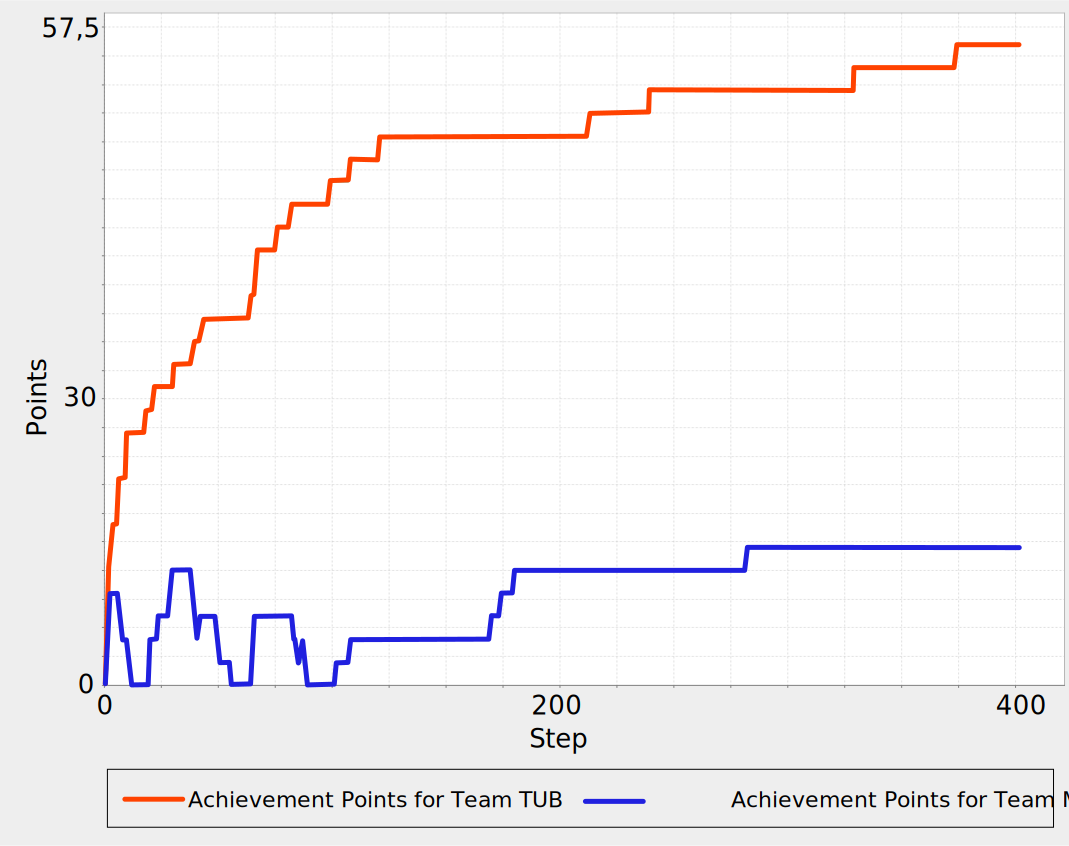
\includegraphics[width=300px]{images/AchievementPoints.png}
	\caption{MAPC 2014 result}
	\label{dis:achievement_points}
\end{figure}
It looks like that this is a huge drawback because achievement points earned at some point count into every future step score. But compared to the number of points awarded for zones, this is only a minor fraction of the step score. As it can be seen in figure \autoref{dis:ZonesScoresAndAchievementPoints} the spending of achievement points paid off since our upgraded saboteur agents hindered the enemy agents from building high valued zones. It was worth spending the achievement points for the purpose of attacking and disturbing the other team because the amount of potential zone points they would have earned without being attacked, is probably much higher than the amount of achievement points team "MaKo" spent for upgrades.
\begin{figure}[h]
	\centering
	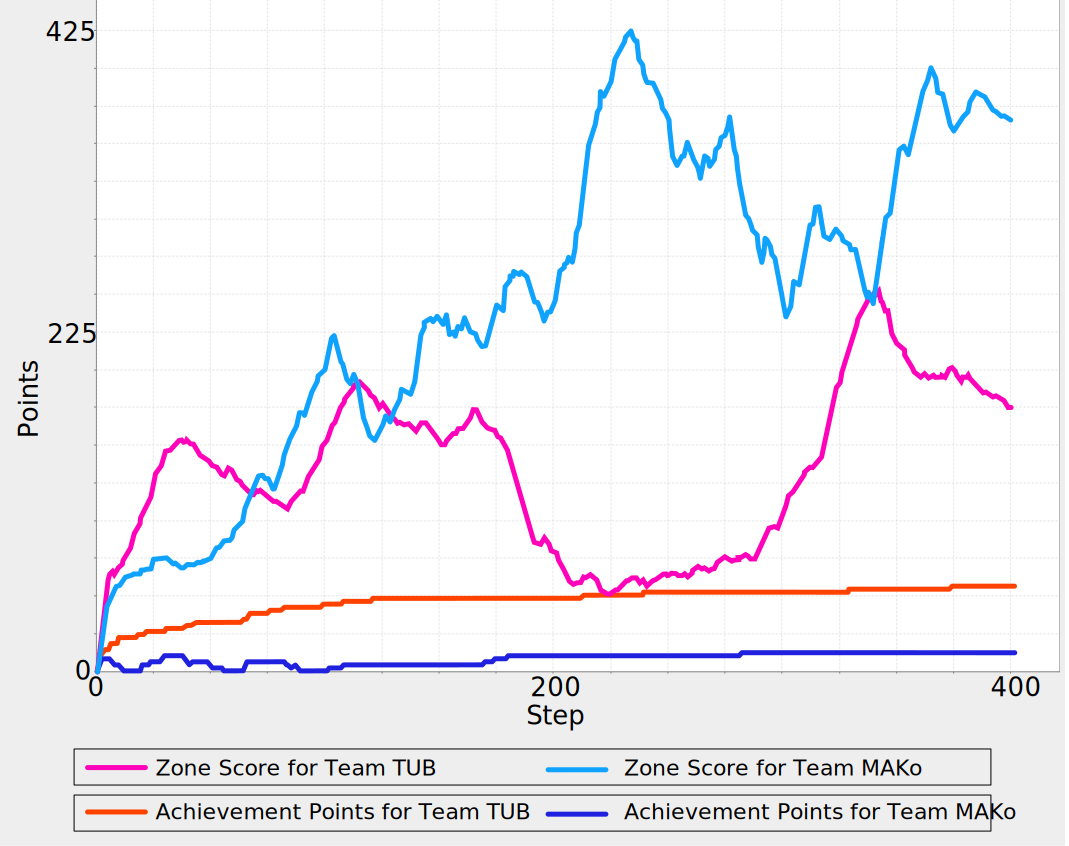
\includegraphics[width=300px]{images/ZonesScoresAndAchievementPoints.png}
	\caption{MAPC 2014 result}
	\label{dis:ZonesScoresAndAchievementPoints}
\end{figure}
At the end of the tournament team "MaKo" scored second with a total of 18 points. The winner 2014 was, for three times in a row now, the team from the USFC. The final results are shown in~\autoref{tab:mapc2014results}.
\begin{table}[ht]
\centering
\caption{The results of the 2014 MAPC. Each team played three matches against every other team, and winning a match awarded 3 points.}
\label{tab:mapc2014results}
\begin{tabular}{@{}lllll@{}}
\toprule
Pos. & Team name      & Score            & Difference            & Points \\ \midrule
1    & SMADAS-UFSC    & 1180662 : 654624 & \phantom{-}526038     & 33     \\
2    & MAKo           & 617086 : 776868  & -15782                & 18     \\
3    & TUB            & 904874 : 872399  & \phantom{-}32475      & 15     \\
4    & TheWonderbolts & 711001 : 1014669 & -303668               & 15     \\
5    & GOAL-DTU       & 653178 : 748241  & -95063                & 9      \\ \bottomrule
\end{tabular}
\end{table}
Statistics of all the individual games can be found in the appendix.[reference here!!!!]

Team "MaKo" lost every second game against each opponent due to the fact that for some reason the repairer agents weren't able to repair. The reason behind this was not obvious to the team. Summarizing the matches, team "MaKo" was capable of exploring the map, building local optima zones, dealing with disabled agents and attacking the opponent. A thing that could be improved is the zoning behaviour. Due to the fact that zones were broken up on a regular basis, zones with a high value sometimes were discarded even when there was no need to do that. Also no handling of edge cases has been implemented which could improve zoning in the sense that the actual number of agents needed to build that zone could be less than the number calculated by our algorithm. But the general idea regarding small zone forming was good. Because one big zone is easy to disturb, having some small high value zones was quite effective to not provide the enemy with an easy target. Like already mentioned a strategy that worked out well, was the approach to upgrade the visibility range and the strength of one saboteur agent significantly. In all matches the it was able to disable enemy agents many times and therefore disturb zones and keep the enemy repairers busy, which kept them away from building zones. 

% TODO: these are from the TOC:
%What place did we rank? How did the others do? Analyse our matches shortly and point out problems we faced, how we tackled them and point out what had gone well.


\subsection{Lessons learned$^{\odot}$}
None of the "MaKo" team member had experience with Jason as a programming language before the research lab.
The first thing that caused problems was that Jason was quite slow, especially when it comes to communication between agents.
Since agents most times needed some information from others and could not continue with their reasoning until this information was given, communication was a extreme bottleneck.
Extreme delay was observed when the group tried to exchange information about the graph.
The first approach was to communicate everything that an agent perceives, while exploring the graph, to every other agent.
The reason behind this was to have every agent store the full knowledge about the until then explored (sub-)graph.
This course of action was quickly discarded, because agents were not able to do actions while processing all the incoming messages.
The next attempt to reduce communication was to implement a so called "cartographer" agent.
The purpose of this agent was to have an additionally agent in the background that gathers all the information about the map that all 28 agents perceive.
With that cartographer agent the amount of communication was reduced and agents could act like intended, because now they just sent their percepts to the cartographer agent and they had not to deal with incoming messages of the other 27 agents.
The drawback of this approach revealed when it came to querying the cartographer agent for information, for instance when an agent wanted to know if a vertex was already surveyed or how he could reach given vertex.
Like it was noticed before, processing the received messages is quite slow and so it happened that the cartographer agent was not able to handle messages in time.
It occurred that agents asked about some specific vertex which the cartographer agent should have known about (because some other agent already informed him about that particular vertex) and they got no answer due to the fact that the cartographer agent hadn't processed the message yet.
That's why this approach was also discarded.
The next idea, which worked in the end, was to use a Java object, the so called "map agent", for the purpose of storing and processing graph information.
Internal actions were used to obtain the required information about the graph.
For instance the internal action "getBestHopToVertex" calculates the shortest path and returns, for a given target node, the next vertex where the agent has to go to.
Another issue that arose initially during the contest was that if a Term in Jason contains a dash, it is interpreted as a Number.
We observed this during our first match against a team that had a dash in its name.
The result was that we were not able to distinguish between friendly and enemy agents.
We immediately fixed it, so that in the next matches we took this possibility of having a dash in the team name into account.

% TODO: these are from the TOC
%Here we could explain what was working well and what was troublesome.  Java: fast.  AS(L): slow and hard for us to program.  Communication: extreme bottleneck.  Also we could note that all this would need much more time and preparation (or a team that is more familiar with agent programming).  %We can illustrate this with our approaches of a dedicated cartographer agent and the node agents.  We might also illustrate further failed approaches.



\bibliographystyle{../template/splncs03}
%\clearpage
\bibliography{content/sources}
\end{document}
